\title{POO - Herança Múltipla}

\author{Prof. Gabriel Rodrigues Caldas de Aquino}

\institute
{
    gabrielaquino@ic.ufrj.br\\
    
    Instituto de Computação -
    Universidade Federal do Rio de Janeiro % Your institution for the title page
}
\date{Compilado em: \\ \today} % Date, can be changed to a custom date

%----------------------------------------------------------------------------------------
%    PRESENTATION SLIDES
%----------------------------------------------------------------------------------------

%------------------------------------------------
\section{Revisão Inicial}
%------------------------------------------------

\begin{frame}
    % Print the title page as the first slide
    \titlepage
\end{frame}
%------------------------------------------------






\begin{frame}{Herança Múltipla em Python - Conceito}

\begin{block}{Definição}
Em Python, uma classe pode herdar de mais de uma classe base:  
\texttt{class Cachorro(Animal, Mamifero):}  

A classe derivada herda todos os atributos e métodos (públicos e protegidos) de todas as classes base.
\end{block}


\end{frame}


\begin{frame}{Herança Múltipla em Python - Conceito}


\begin{block}{Ordem de Resolução de Métodos (MRO)}
\begin{itemize}
    \item O método \texttt{mro()}, herdado de \texttt{object}, mostra a Ordem de Resolução de Métodos (Method Resolution Order - MRO) de uma classe.
    \item Se múltiplas classes base possuem um método ou atributo com o mesmo nome, o da classe mais à esquerda na herança prevalece.
\end{itemize}
\end{block}





\end{frame}




\begin{frame}{Herança Múltipla}
    \centering
    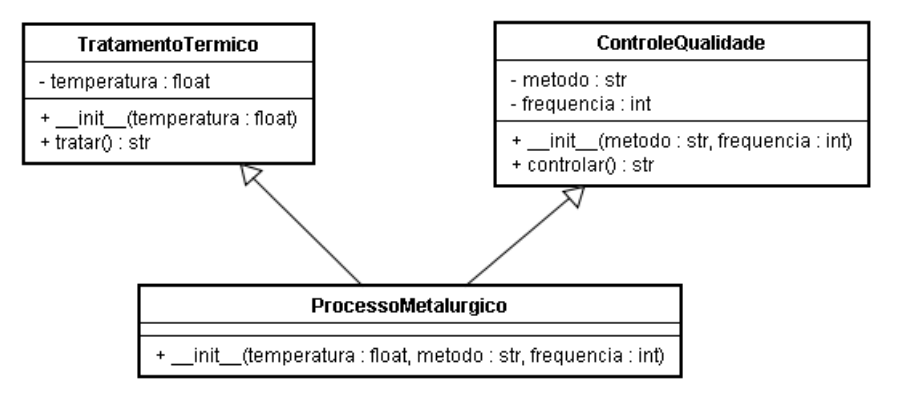
\includegraphics[width=0.8\textwidth]{Images/heranca-multipla.png}
\end{frame}

\begin{frame}{Herança Múltipla - Cenário: Processos Metalúrgicos}
Um processo metalúrgico envolve várias etapas, e duas delas são:

\begin{itemize}
    \item \textbf{Tratamento térmico:} define como o material é aquecido e resfriado para alterar suas propriedades (dureza, resistência, etc.).
    \item \textbf{Controle de qualidade:} garante que o produto final atenda aos padrões, fazendo medições, testes e inspeções.
\end{itemize}


\texttt{TratamentoTermico} e \texttt{ControleDeQualidade} são classes independentes:
\begin{itemize}
    \item Representam aspectos diferentes e podem ser aplicados em outros contextos. 
\end{itemize}


\texttt{ProcessoMetalurgico} herda dessas duas:
\begin{itemize}
    \item Processo metalúrgico envolve tanto tratamento térmico quanto validação de qualidade.  
\end{itemize}


A herança múltipla: 
\begin{itemize}
    \item Permite que a classe final tenha os métodos e atributos de ambas, compondo o comportamento necessário.
\end{itemize}
\end{frame}

\begin{frame}[fragile]{Implementação do exemplo - Processos Metalúrgicos}
\begin{figure}
    \centering
    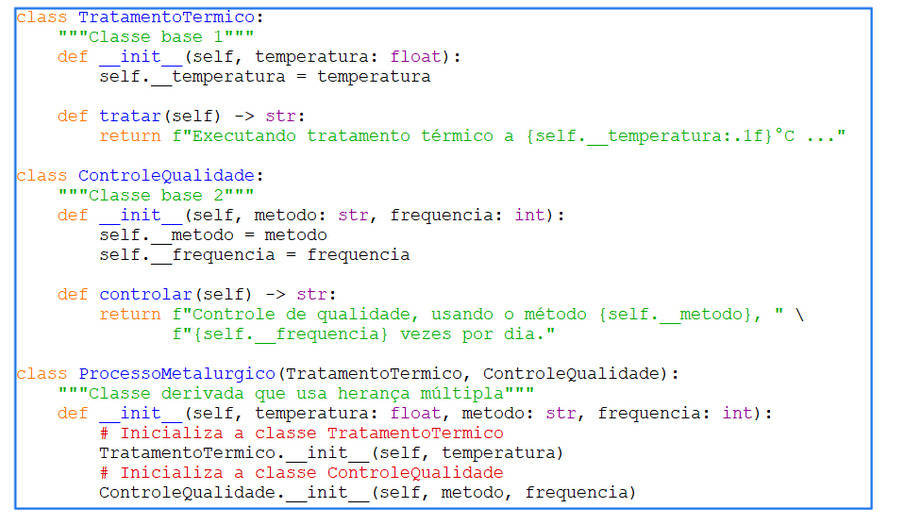
\includegraphics[width=0.9\linewidth]{Images/tratamento-processo-qualidade.png}


\end{figure}
    
\end{frame}



\begin{frame}{Herança Múltipla em Python - Como Funciona}

\begin{block}{Funcionamento}
\begin{itemize}
    \item Uma classe derivada pode herdar de mais de uma classe base.
    \item Todos os atributos e métodos (públicos e protegidos) das classes base são herdados.
    \item Quando várias classes base possuem métodos ou atributos com o mesmo nome:
    \begin{itemize}
        \item O método ou atributo da classe mais à esquerda na definição da herança é usado.
    \end{itemize}
    \item O Python utiliza a \textbf{Ordem de Resolução de Métodos (MRO)} para determinar qual método será chamado.
    \item O método \texttt{mro()} da \textbf{classe} mostra essa ordem.
\end{itemize}
\end{block}


\end{frame}

\begin{frame}{Herança Múltipla em Python - Resumo}

\begin{itemize}
    \item Herança múltipla permite reaproveitar código de diversas classes
    \item \textbf{Importante}: entender a MRO para evitar comportamentos inesperados quando houver métodos com o mesmo nome.
\end{itemize}



\end{frame}




\begin{frame}[fragile]{Herança Múltipla em Python - Exemplo Prático}
\small
\begin{verbatim}
class A:
    def metodo1(self):
        print("Metodo1 - Classe A")  
    def metodoA2(self):
        print("MetodoA2 - Classe A")    
class B:
    def metodo1(self):
        print("Metodo1 - Classe B")
    def metodoB2(self):
        print("MetodoB2 - Classe B")    
class C(A, B):
    pass
c = C()
c.metodo1()
c.metodoA2()
c.metodoB2()
print(C.mro())  # Mostra a ordem de herança
\end{verbatim}
\end{frame}

\begin{frame}{Entendendo a saída}
\begin{figure}
    \centering
    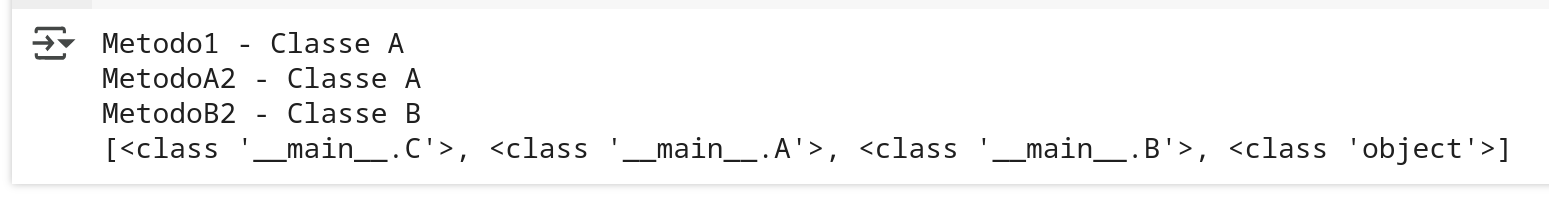
\includegraphics[width=0.9\linewidth]{Images/mro-saida-2.png}

\end{figure}


Explicação detalhada:
    \begin{itemize}
        \item Python segue a ordem do MRO: C → A → B
         \item        Encontra metodo1() primeiro na Classe A
         \item   c.metodoA2() → só existe na Classe A, então o  Python encontra e executa normalmente
          \item    c.metodoB2() → só existe na Classe B, então o  Python encontra e executa normalmente
          \item  C.mro() → Mostra a ordem de resolução de métodos
    \end{itemize}



    
\end{frame}

\begin{frame}[fragile]{E se eu quiser executar em uma ordem diferente?}
\footnotesize
    \begin{verbatim}
class CLASS_A:
    nome = "Classe A"
    def metodo1(self):
        print(f"Classe A fala: {self.nome}")  
class CLASS_B:
    nome = "Classe B"
    def metodo1(self):
        print(f"Classe B fala: {self.nome}")
class CLASS_C(CLASS_A, CLASS_B):
    nome = "Classe C"
    pass
var_a = A()
var_b = B()
var_c = C()
var_a.metodo1()
var_b.metodo1()
var_c.metodo1()
print(CLASS_C.mro())
CLASS_B.metodo1(var_c)  
    \end{verbatim}
\end{frame}

\begin{frame}{Herança Múltipla – método \texttt{super()}}

\begin{block}{Uso de \texttt{super()}}
\begin{itemize}
    \item O método \texttt{super()} permite chamar métodos ou construtores da superclasse.
    \item Em herança múltipla, o \texttt{super()} segue a Ordem de Resolução de Métodos (MRO).
\end{itemize}
\end{block}

\begin{block}{Recomendação em herança múltipla}
\begin{itemize}
    \item Se os métodos das superclasses tiverem parâmetros diferentes, pode haver conflito.
    \item Nesses casos, é mais seguro usar a chamada explícita:  
    \texttt{NomeDaSuperClasse.metodo(self, ...)}  
    ao invés de \texttt{super().metodo(...)}.
    \item Isso garante que cada classe receba os parâmetros corretos e evita erros de inicialização.

    \item \texttt{super()} é útil para reutilizar métodos da superclasse.  
    \item Em herança múltipla complexa, chamadas explícitas podem ser mais claras e seguras.
    \end{itemize}
\end{block}

\end{frame}


\begin{frame}[fragile]{Herança Múltipla - Exemplo Prático: Hidrocarro}


\scriptsize
\begin{verbatim}
class Carro:
    def __init__(self, rodas):
        self.rodas = rodas
    def dirigir(self):
        print(f"Dirigindo o carro com {self.rodas} rodas.")
class Barco:
    def __init__(self, tamanho):
        self.tamanho = tamanho
    def navegar(self):
        print(f"Navegando no barco de {self.tamanho} metros.")
class Hidrocarro(Carro, Barco):
    def __init__(self, rodas, tamanho):
        Carro.__init__(self, rodas)
        Barco.__init__(self, tamanho)
    def mostrar_info(self):
        print(f"Hidrocarro com {self.rodas} rodas e {self.tamanho} metros de comprimento.")
h = Hidrocarro(4, 7)
h.dirigir()
h.navegar()
h.mostrar_info()
\end{verbatim}
\end{frame}